\section{Jacobian Matrix Development for Magic Formula Tire Model}

\subsection{Ground}

The ground plane is (locally) described by a reference point and a normal unit vector, represented in the global reference frame as $\mathbf{q}$ and $\mathbf{n}$, respectively. To simplify the derivation (for now), a constant flat plane is considered, thus $\mathbf{q}$ and $\mathbf{n}$ are constant vectors equal to:
\begin{equation}
    \label{eq:assumptions}
    \mathbf{q} = \mathbf{0}\hspace{1cm}\mathbf{n} = \begin{bmatrix}
        0 & 0 & 1
    \end{bmatrix}^T
\end{equation}

\subsection{Wheel Hub and Wheel Rim}

Two nodes are needed to fully describe the contact point kinematics. The wheel hub node (static/dynamic, non-rotating) and the rim node (dynamic, rotating). The wheel hub and rim are only allowed to rotate around a fixed axis, indicated as $\tilde{s}$ in the local reference frame of the wheel hub.

The wheel hub node position is $\mathbf{w}_H$, and its orientation matrix is denoted as $\mathbf{R}_H$. The rim angular velocity is denoted by $\boldsymbol{\omega}_R$
The first task is to compute the wheel spin axis unit vector, which is obtained as follows:
\begin{equation}
    \mathbf{s} = \mathbf{R}_H \tilde{\mathbf{s}} = \mathbf{R}_H \begin{bmatrix}
        0 & 1 & 0
    \end{bmatrix}^T
\end{equation}
Two other vectors are introduced to identify the forward ($\mathbf{l}$) and transverse ($\mathbf{t}$) directions relative to the wheel.
\begin{equation}
    \begin{split}
        \mathbf{l} &= \frac{\mathbf{s} \times \mathbf{n}}{||\mathbf{s} \times \mathbf{n}||}\\
        \mathbf{t} &= \mathbf{n} \times \mathbf{l}
    \end{split}
\end{equation}

\section{Slip Quantities}

The following three velocity components make the definition of the slip quantities easier:
\begin{equation}
    \begin{split}
        v_x &= \mathbf{l} \cdot \dot{\mathbf{w}}_H\\
        v_y &= \mathbf{t} \cdot \dot{\mathbf{w}}_H\\
        v_s &= \mathbf{l} \cdot \left(\boldsymbol{\omega}_R \times r_e \mathbf{n}\right)\\
    \end{split}
\end{equation}
$r_e$ is the (constant, for now) effective rolling radius.
Longitudinal and lateral slips require particular care to avoid numerical instability as longitudinal speed tends towards zero. As commonly suggested in vehicle dynamics literature, ad hoc definitions of slip angle and slip ratio are adopted below a given speed threshold ($v_{x, \text{LOW}}$), denoted as $\alpha_L$ and $\kappa_L$, to avoid division by zero. Above that threshold, the standard definitions are applied, $\alpha_H$ and $\kappa_H$.
\begin{equation}
    \begin{split}
        \alpha_H &= \arctan\left(\frac{v_y}{v_x}\right)\\
        \kappa_H &= \frac{v_s}{v_x} - 1
    \end{split}
\end{equation}
\begin{equation}
    \begin{split}
        \alpha_L &= v_y\\
        \kappa_L &= v_s - v_x
    \end{split}
\end{equation}
The two functions
\begin{equation}
    \kappa = 
    \begin{cases} 
        \kappa_L & \text{if } |v_x| \leq v_{x,\text{LOW}}, \\
        \kappa_H & \text{if } |v_x| > v_{x,\text{LOW}}, \\
    \end{cases}
\end{equation}
\begin{equation}
    \alpha = 
    \begin{cases} 
        \alpha_L & \text{if } |v_x| \leq v_{x,\text{LOW}}, \\
        \alpha_H & \text{if } |v_x| > v_{x,\text{LOW}}, \\
    \end{cases}
\end{equation} 
are not continuous at $v_x = v_{x,\text{LOW}}$. To smoothly transition between the two definitions, a function $\chi$ is introduced. This also allows to obtain a single continuous function which can be differentiated and easily included in the model Jacobian matrix. The parameter $v_{x, \text{DMP}}$ allows to tune how quickly the transition between low speed and high speed state happens.
\begin{equation}
    \chi = \frac{1}{2}\left[\tanh\left(\frac{|v_x| - v_{x, \text{LOW}}}{v_{x, \text{DMP}}}\right) + 1\right]
\end{equation}
The expression for the derivative of $\chi$, needed in the Jacobian matrix, is reported in \ref{ss:derivatives}
\begin{figure}
    \centering
    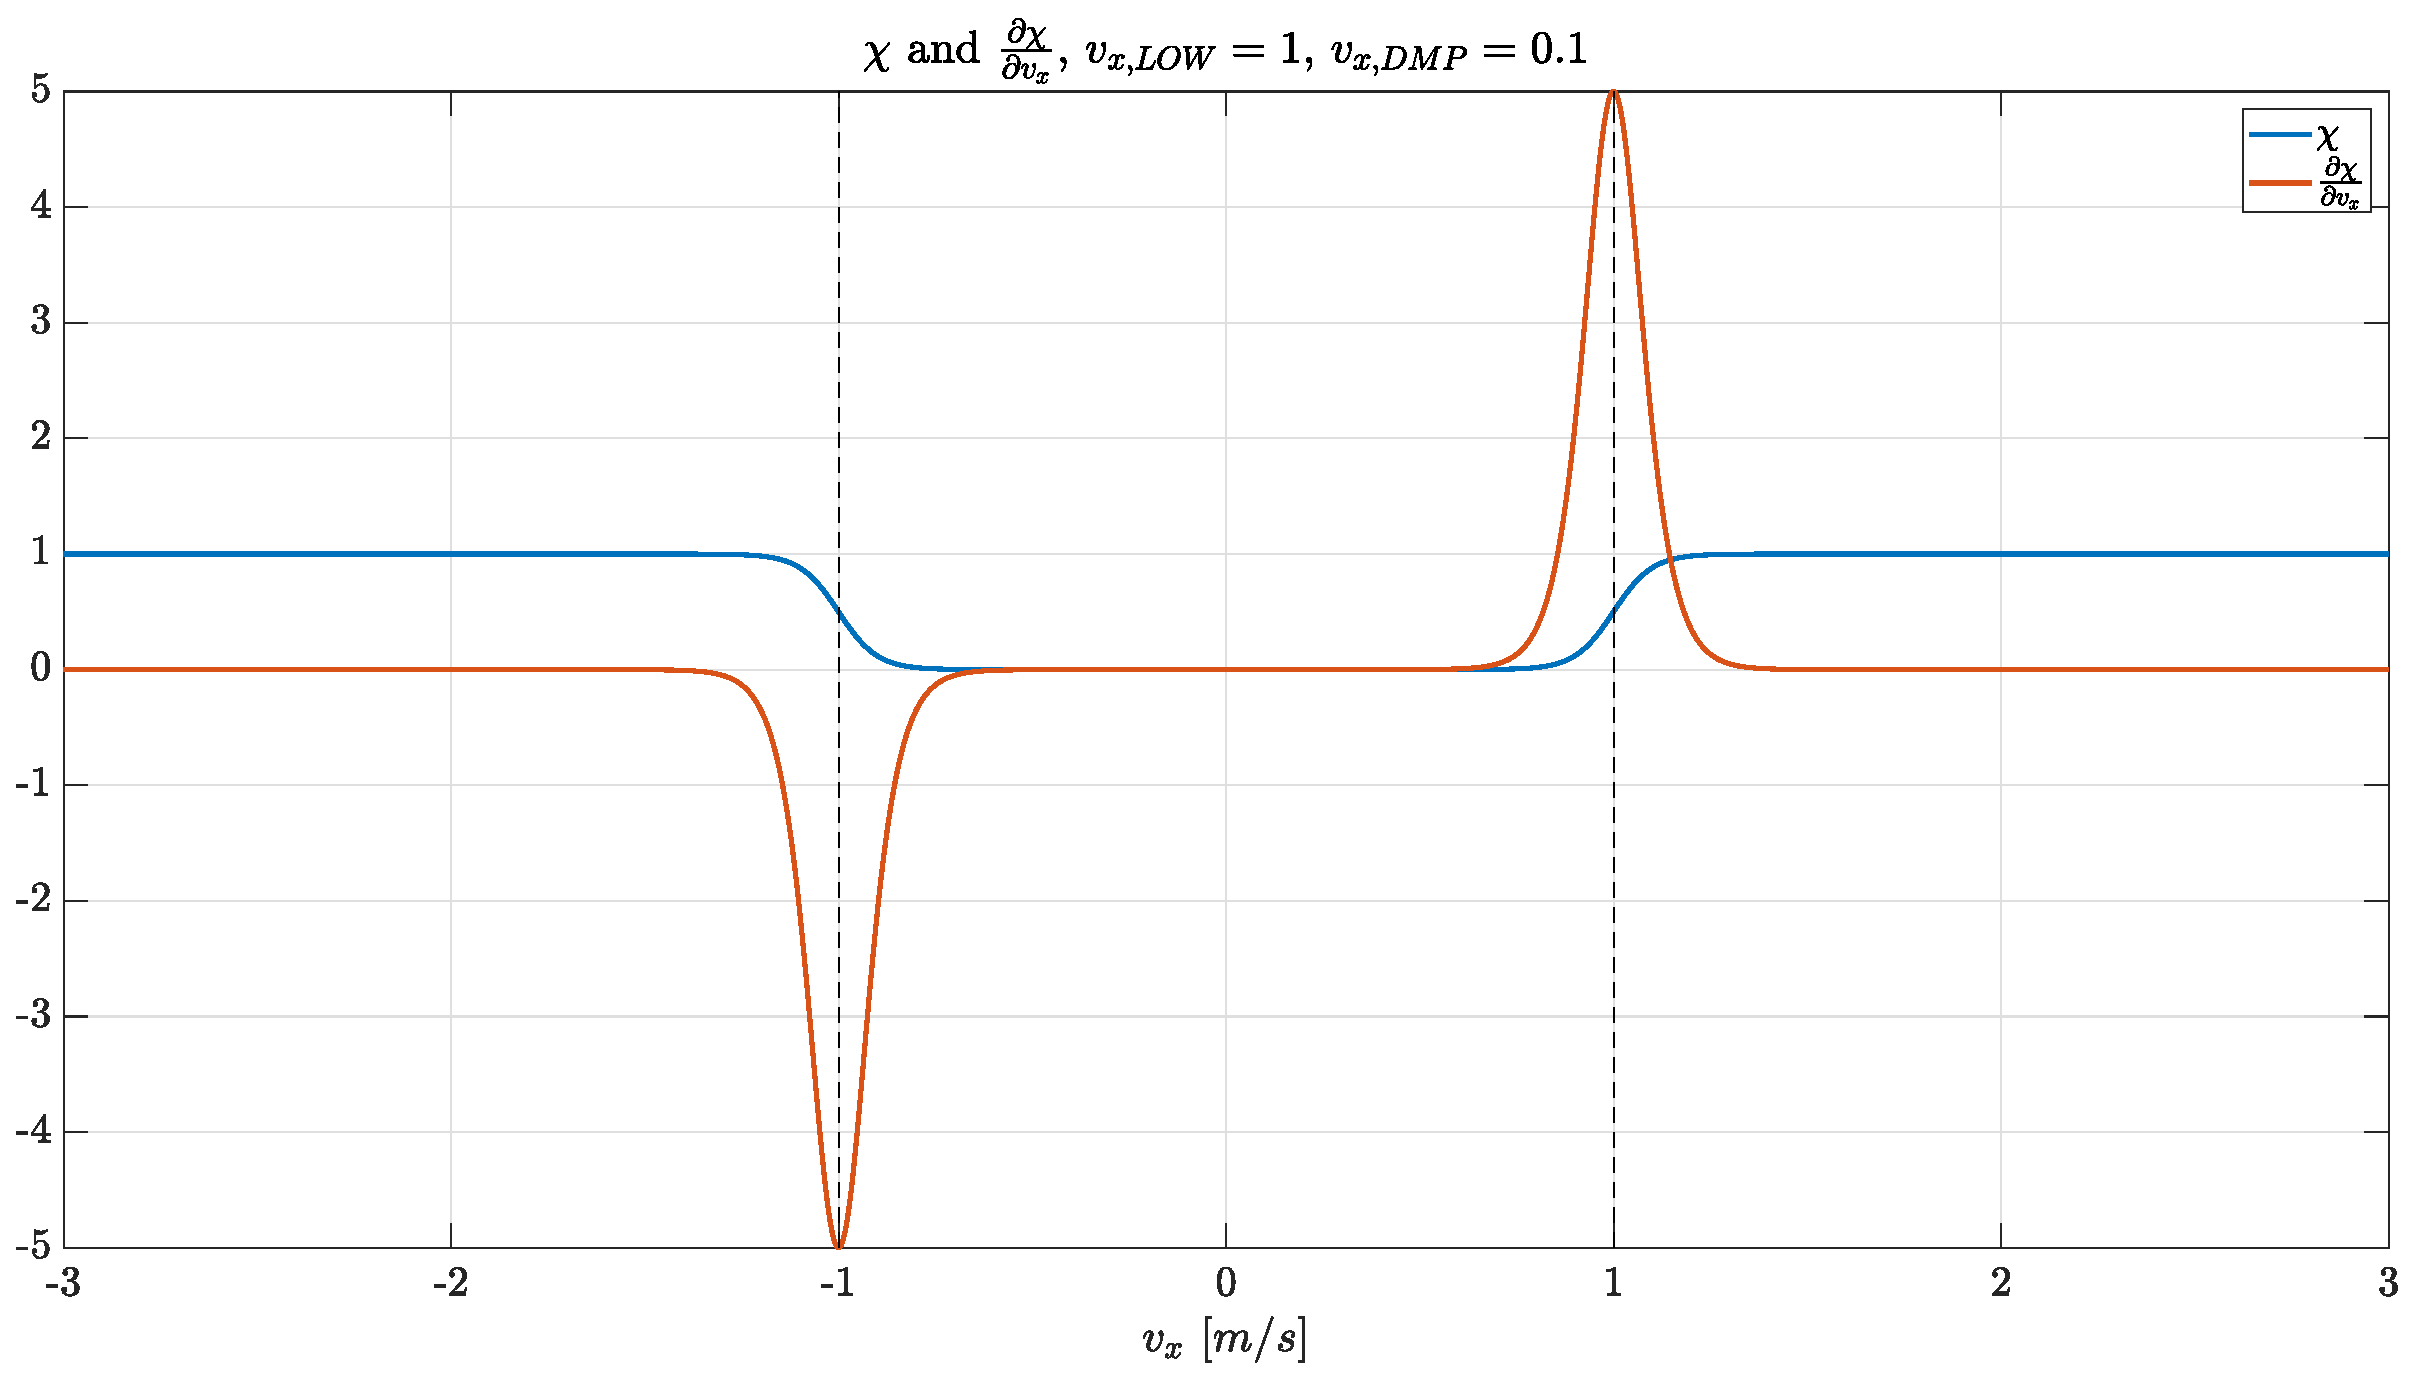
\includegraphics[width=1\textwidth]{MFtirePlots/transition.eps}
    \caption{$\chi$ and $\frac{\partial{\chi}}{\partial{v_x}}$}
\end{figure}
Finally, slip angle and slip ratio are expressed as:
\begin{equation}
    \begin{split}
        \alpha &= \chi \alpha_H + (1-\chi) \alpha_L\\
        \kappa &= \chi \kappa_H + (1-\chi) \kappa_L\\
    \end{split}
\end{equation}

\section{Radial Deflection}

The loaded radius is calculated as 
\begin{equation}
    r = \mathbf{w} \cdot \mathbf{n}
\end{equation}

\section{Tire forces}

At this point, the forces (which must be applied on the wheel hub) can be calculated:
\begin{equation}
    \begin{split}
        F_z &= k_t\left(r_0 - r\right)\\
        F_x &= F_z \mu_x(\kappa)\\
        F_y &= F_z \mu_y(\alpha)
    \end{split}
\end{equation}
Where
\begin{equation}
    \begin{split}
        \mu_x(\kappa) &= D_x\sin(C_x\arctan(B_x\kappa-E_x(B_x\kappa-\arctan(B_x\kappa))))\\
        \mu_y(\alpha) &= D_y\sin(C_y\arctan(B_y\alpha-E_y(B_y\alpha-\arctan(B_y\alpha))))\\
    \end{split}
\end{equation}
The total tire force can be obtained as:
\begin{equation}
    \mathbf{F} = F_z \mathbf{n} + F_x \mathbf{l} + F_y \mathbf{t}
\end{equation}
And finally, the transport moments
\begin{equation}
    \mathbf{M} = -r \mathbf{n} \times \mathbf{F}
\end{equation}

\section{Jacobian Components}
Subscript H refers to the hub, while subscript R to the rim.
\subsection{Vectors Perturbations}
\begin{equation}
    \begin{split}
        \Delta \mathbf{s} &= \boldsymbol{\theta}_{\Delta H} \times \mathbf{s}\\
        &= \left[\mathbf{s} \times ^T\right] \boldsymbol{\theta}_{\Delta H}
    \end{split}
\end{equation}
\begin{equation}
    \begin{split}
        \Delta \mathbf{l} &= \left[\frac{\mathbf{n}\times^T}{||\mathbf{s}\times\mathbf{n}||} + \frac{\left(\mathbf{s}\times\mathbf{n}\right)\left(\mathbf{s}\times\mathbf{n}\right)^T\mathbf{n}\times}{||\mathbf{s}\times\mathbf{n}||^3}\right] \Delta \mathbf{s}\\
        &= \left[\frac{\mathbf{n}\times^T}{||\mathbf{s}\times\mathbf{n}||} + \frac{\left(\mathbf{s}\times\mathbf{n}\right)\left(\mathbf{s}\times\mathbf{n}\right)^T\mathbf{n}\times}{||\mathbf{s}\times\mathbf{n}||^3} \mathbf{J}_\mathbf{s} \right] \boldsymbol{\theta}_{\Delta H}\\
        &= \mathbf{J}_\mathbf{l} \boldsymbol{\theta}_{\Delta H}
    \end{split}
\end{equation}
\begin{equation}
    \begin{split}
        \Delta \mathbf{t} &= \mathbf{n} \times \Delta \mathbf{l}\\
        &= \left[\mathbf{n} \times \mathbf{J}_\mathbf{l} \right]\boldsymbol{\theta}_{\Delta H}\\
        &= \mathbf{J}_\mathbf{t} \boldsymbol{\theta}_{\Delta H}
    \end{split}
\end{equation}
\subsection{Velocities Perturbations}
\begin{equation}
    \begin{split}
        \Delta v_x &= \frac{\partial{v_x}}{\partial{\mathbf{l}}}\Delta \mathbf{l} + \frac{\partial{v_x}}{\partial{\dot{\mathbf{w}}_H}}\Delta {\dot{\mathbf{w}}}_H\\
        &= \left[\dot{\mathbf{w}}_H^T \mathbf{J}_\mathbf{l}\right] \boldsymbol{\theta}_{\Delta H} + \left[\mathbf{l}^T\right] \Delta {\dot{\mathbf{w}}}_H\\
        &= \mathbf{J}_{{v_x}_{\boldsymbol{\theta}_{\Delta H}}} \boldsymbol{\theta}_{\Delta H} + \mathbf{J}_{{v_x}_{\dot{\mathbf{w}}_H}} \Delta {\dot{\mathbf{w}}}_H
    \end{split}
\end{equation}
\begin{equation}
    \begin{split}
        \Delta v_y &= \frac{\partial{v_y}}{\partial{\mathbf{t}}}\Delta \mathbf{t} + \frac{\partial{v_y}}{\partial{\dot{\mathbf{w}}_H}}\Delta {\dot{\mathbf{w}}}_H\\
        &= \left[\dot{\mathbf{w}}_H^T \mathbf{J}_\mathbf{t}\right] \boldsymbol{\theta}_{\Delta H} + \left[\mathbf{t}^T\right] \Delta {\dot{\mathbf{w}}}_H\\
        &= \mathbf{J}_{{v_y}_{\boldsymbol{\theta}_{\Delta H}}} \boldsymbol{\theta}_{\Delta H} + \mathbf{J}_{{v_y}_{\dot{\mathbf{w}}_H}} \Delta {\dot{\mathbf{w}}}_H
    \end{split}
\end{equation}
\begin{equation}
    \begin{split}
        \Delta v_s &= \frac{\partial{v_s}}{\partial{\mathbf{l}}}\Delta \mathbf{l} + \frac{\partial{v_s}}{\partial{\boldsymbol{\omega}_R}}\Delta \boldsymbol{\omega}_R\\
        &= \left[\left(\boldsymbol{\omega}_R \times r_e \mathbf{n}\right)^T \mathbf{J}_\mathbf{l}\right] \boldsymbol{\theta}_{\Delta H} + \left[r_e \mathbf{l}^T \mathbf{n} \times ^T\right] \Delta \boldsymbol{\omega}_R\\
        &= \mathbf{J}_{{v_s}_{\boldsymbol{\theta}_{\Delta H}}} \boldsymbol{\theta}_{\Delta H} + \mathbf{J}_{{v_s}_{\boldsymbol{\omega}_R}} \Delta \boldsymbol{\omega}_R
    \end{split}
\end{equation}
\subsection{Slip Quantities Perturbations}
\begin{equation}
    \begin{split}
        \Delta \alpha_H &= \frac{\partial{\alpha}}{\partial{v_y}} \Delta v_y + \frac{\partial{\alpha}}{\partial{v_x}} \Delta v_x\\
        &= \frac{v_x}{v_x^2 + v_y^2} \left(\mathbf{J}_{{v_y}_{\boldsymbol{\theta}_{\Delta H}}} \boldsymbol{\theta}_{\Delta H} + \mathbf{J}_{{v_y}_{\dot{\mathbf{w}}_H}} \Delta {\dot{\mathbf{w}}}_H\right) - \frac{v_y}{v_x^2 + v_y^2} \left(\mathbf{J}_{{v_x}_{\boldsymbol{\theta}_{\Delta H}}} \boldsymbol{\theta}_{\Delta H} + \mathbf{J}_{{v_x}_{\dot{\mathbf{w}}_H}} \Delta {\dot{\mathbf{w}}}_H\right)\\
        &= \left[\frac{v_x}{v_x^2 + v_y^2} \mathbf{J}_{{v_y}_{\boldsymbol{\theta}_{\Delta H}}} - \frac{v_y}{v_x^2 + v_y^2}\mathbf{J}_{{v_x}_{\boldsymbol{\theta}_{\Delta H}}}\right] \boldsymbol{\theta}_{\Delta H}\\
        &+ \left[\frac{v_x}{v_x^2 + v_y^2} \mathbf{J}_{{v_y}_{\dot{\mathbf{w}}_H}} - \frac{v_y}{v_x^2 + v_y^2}\mathbf{J}_{{v_x}_{\dot{\mathbf{w}}_H}}\right] \Delta {\dot{\mathbf{w}}}_H\\
        &= \mathbf{J}_{\alpha_{H, \boldsymbol{\theta}_{\Delta H}}}\boldsymbol{\theta}_{\Delta H} + \mathbf{J}_{\alpha_{H, \dot{\mathbf{w}}_H}}\Delta {\dot{\mathbf{w}}}_H\\
        \Delta \kappa_H &= \frac{\partial{\kappa}}{\partial{v_s}} \Delta v_s + \frac{\partial{\kappa}}{\partial{v_x}} \Delta v_x\\
        &= \frac{1}{v_x} \left(\mathbf{J}_{{v_s}_{\boldsymbol{\theta}_{\Delta H}}} \boldsymbol{\theta}_{\Delta H} + \mathbf{J}_{{v_s}_{\boldsymbol{\omega}_R}} \Delta \boldsymbol{\omega}_R\right) - \frac{v_s}{v_x^2} \left(\mathbf{J}_{{v_x}_{\boldsymbol{\theta}_{\Delta H}}} \boldsymbol{\theta}_{\Delta H} + \mathbf{J}_{{v_x}_{\dot{\mathbf{w}}_H}} \Delta {\dot{\mathbf{w}}}_H\right) \\
        &= \left[\frac{1}{v_x} \mathbf{J}_{{v_s}_{\boldsymbol{\theta}_{\Delta H}}} - \frac{v_s}{v_x^2} \mathbf{J}_{{v_x}_{\boldsymbol{\theta}_{\Delta H}}}\right] \boldsymbol{\theta}_{\Delta H}\\
        &+ \left[\frac{1}{v_x} \mathbf{J}_{{v_s}_{\boldsymbol{\omega}_R}}\right] \Delta \boldsymbol{\omega}_R\\
        &+ \left[- \frac{v_s}{v_x^2} \mathbf{J}_{{v_x}_{\dot{\mathbf{w}}_H}}\right]\Delta {\dot{\mathbf{w}}}_H\\
        &= \mathbf{J}_{\kappa_{H, \boldsymbol{\theta}_{\Delta H}}}\boldsymbol{\theta}_{\Delta H} + \mathbf{J}_{\kappa_{H, \boldsymbol{\omega}_R}}\Delta \boldsymbol{\omega}_R + \mathbf{J}_{\kappa_{H, \dot{\mathbf{w}}_H}}\Delta {\dot{\mathbf{w}}}_H
    \end{split}
\end{equation}
\begin{equation}
    \begin{split}
        \Delta \alpha_L &= \Delta v_y\\
        &= \mathbf{J}_{{v_y}_{\boldsymbol{\theta}_{\Delta H}}} \boldsymbol{\theta}_{\Delta H} + \mathbf{J}_{{v_y}_{\dot{\mathbf{w}}_H}} \Delta {\dot{\mathbf{w}}}_H\\
        &= \mathbf{J}_{\alpha_{L, \boldsymbol{\theta}_{\Delta H}}}\boldsymbol{\theta}_{\Delta H} + \mathbf{J}_{\alpha_{L, \dot{\mathbf{w}}_H}}\Delta {\dot{\mathbf{w}}}_H\\
        \Delta \kappa_L &= \Delta v_s - \Delta v_x\\
        &= \left(\mathbf{J}_{{v_s}_{\boldsymbol{\theta}_{\Delta H}}} \boldsymbol{\theta}_{\Delta H} + \mathbf{J}_{{v_s}_{\boldsymbol{\omega}_R}} \Delta \boldsymbol{\omega}_R\right) - \left(\mathbf{J}_{{v_x}_{\boldsymbol{\theta}_{\Delta H}}} \boldsymbol{\theta}_{\Delta H} + \mathbf{J}_{{v_x}_{\dot{\mathbf{w}}_H}} \Delta {\dot{\mathbf{w}}}_H\right)\\
        &= \left[\mathbf{J}_{{v_s}_{\boldsymbol{\theta}_{\Delta H}}} - \mathbf{J}_{{v_x}_{\boldsymbol{\theta}_{\Delta H}}} \right] \boldsymbol{\theta}_{\Delta H} + \left[\mathbf{J}_{{v_s}_{\boldsymbol{\omega}_R}}\right] \Delta \boldsymbol{\omega}_R - \left[\mathbf{J}_{{v_x}_{\dot{\mathbf{w}}_H}}\right] \Delta {\dot{\mathbf{w}}}_H\\
        &= \mathbf{J}_{\kappa_{L, \boldsymbol{\theta}_{\Delta H}}}\boldsymbol{\theta}_{\Delta H} + \mathbf{J}_{\kappa_{L, \boldsymbol{\omega}_R}}\Delta \boldsymbol{\omega}_R + \mathbf{J}_{\kappa_{L, \dot{\mathbf{w}}_H}}\Delta {\dot{\mathbf{w}}}_H
    \end{split}
\end{equation}
\begin{equation}
    \begin{split}
        \Delta \kappa &= \frac{\partial\kappa}{\partial\chi}\Delta\chi + \frac{\partial\kappa}{\partial\kappa_L}\Delta\kappa_L + \frac{\partial\kappa}{\partial\kappa_H}\Delta\kappa_H \\
        &= \left(\kappa_H - \kappa_L\right)\frac{\partial\chi}{\partial v_x}\left(\mathbf{J}_{{v_x}_{\boldsymbol{\theta}_{\Delta H}}} \boldsymbol{\theta}_{\Delta H} + \mathbf{J}_{{v_x}_{\dot{\mathbf{w}}_H}} \Delta {\dot{\mathbf{w}}}_H\right)\\
        &+ \left(1-\chi\right)\left(\mathbf{J}_{\kappa_{L, \boldsymbol{\theta}_{\Delta H}}}\boldsymbol{\theta}_{\Delta H} + \mathbf{J}_{\kappa_{L, \boldsymbol{\omega}_R}}\Delta \boldsymbol{\omega}_R + \mathbf{J}_{\kappa_{L, \dot{\mathbf{w}}_H}}\Delta {\dot{\mathbf{w}}}_H\right)\\
        &+ \chi\left(\mathbf{J}_{\kappa_{H, \boldsymbol{\theta}_{\Delta H}}}\boldsymbol{\theta}_{\Delta H} + \mathbf{J}_{\kappa_{H, \boldsymbol{\omega}_R}}\Delta \boldsymbol{\omega}_R + \mathbf{J}_{\kappa_{H, \dot{\mathbf{w}}_H}}\Delta {\dot{\mathbf{w}}}_H\right)\\
        &= \left[\left(\kappa_H - \kappa_L\right)\frac{\partial\chi}{\partial v_x}\mathbf{J}_{{v_x}_{\boldsymbol{\theta}_{\Delta H}}} + \left(1-\chi\right)\mathbf{J}_{\kappa_{L, \boldsymbol{\theta}_{\Delta H}}} + \chi \mathbf{J}_{\kappa_{H, \boldsymbol{\theta}_{\Delta H}}}\right] \boldsymbol{\theta}_{\Delta H}\\
        &+ \left[\left(\kappa_H - \kappa_L\right)\frac{\partial\chi}{\partial v_x}\mathbf{J}_{{v_x}_{\dot{\mathbf{w}}_H}} + \left(1-\chi\right)\mathbf{J}_{\kappa_{L, \dot{\mathbf{w}}_H}} + \chi \mathbf{J}_{\kappa_{H, \dot{\mathbf{w}}_H}}\right] \Delta {\dot{\mathbf{w}}}_H\\
        &+ \left[\left(1-\chi\right)\mathbf{J}_{\kappa_{L, \boldsymbol{\omega}_R}} + \chi \mathbf{J}_{\kappa_{H, \boldsymbol{\omega}_R}}\right] \Delta \boldsymbol{\omega}_R\\
        &= \mathbf{J}_{\kappa_{\boldsymbol{\theta}_{\Delta H}}}\boldsymbol{\theta}_{\Delta H} + \mathbf{J}_{\kappa_{\boldsymbol{\omega}_R}}\Delta \boldsymbol{\omega}_R + \mathbf{J}_{\kappa_{\dot{\mathbf{w}}_H}}\Delta {\dot{\mathbf{w}}}_H
    \end{split}
\end{equation}
\begin{equation}
    \begin{split}
        \Delta \alpha &= \frac{\partial\alpha}{\partial\chi}\Delta\chi + \frac{\partial\alpha}{\partial\alpha_L}\Delta\alpha_L + \frac{\partial\alpha}{\partial\alpha_H}\Delta\alpha_H \\
        &= \left(\alpha_H - \alpha_L\right)\frac{\partial\chi}{\partial v_x}\left(\mathbf{J}_{{v_x}_{\boldsymbol{\theta}_{\Delta H}}} \boldsymbol{\theta}_{\Delta H} + \mathbf{J}_{{v_x}_{\dot{\mathbf{w}}_H}} \Delta {\dot{\mathbf{w}}}_H\right)\\
        &+ \left(1-\chi\right)\left(\mathbf{J}_{\alpha_{L, \boldsymbol{\theta}_{\Delta H}}}\boldsymbol{\theta}_{\Delta H} + \mathbf{J}_{\alpha_{L, \dot{\mathbf{w}}_H}}\Delta {\dot{\mathbf{w}}}_H\right)\\
        &+ \chi\left(\mathbf{J}_{\alpha_{H, \boldsymbol{\theta}_{\Delta H}}}\boldsymbol{\theta}_{\Delta H} + \mathbf{J}_{\alpha_{H, \dot{\mathbf{w}}_H}}\Delta {\dot{\mathbf{w}}}_H\right)\\
        &= \left[\left(\alpha_H - \alpha_L\right)\frac{\partial\chi}{\partial v_x}\mathbf{J}_{{v_x}_{\boldsymbol{\theta}_{\Delta H}}} + \left(1-\chi\right)\mathbf{J}_{\alpha_{L, \boldsymbol{\theta}_{\Delta H}}} + \chi \mathbf{J}_{\alpha_{H, \boldsymbol{\theta}_{\Delta H}}}\right] \boldsymbol{\theta}_{\Delta H}\\
        &+ \left[\left(\alpha_H - \alpha_L\right)\frac{\partial\chi}{\partial v_x}\mathbf{J}_{{v_x}_{\dot{\mathbf{w}}_H}} + \left(1-\chi\right)\mathbf{J}_{\alpha_{L, \dot{\mathbf{w}}_H}} + \chi \mathbf{J}_{\alpha_{H, \dot{\mathbf{w}}_H}}\right] \Delta {\dot{\mathbf{w}}}_H\\
        &= \mathbf{J}_{\alpha_{\boldsymbol{\theta}_{\Delta H}}}\boldsymbol{\theta}_{\Delta H} + \mathbf{J}_{\alpha_{\dot{\mathbf{w}}_H}}\Delta {\dot{\mathbf{w}}}_H
    \end{split}
\end{equation}

\subsection{Tire Radius Perturbation}
\begin{equation}
    \begin{split}
        \Delta r &= \Delta \mathbf{w} \cdot \mathbf{n}\\
        &= \mathbf{n}^T \Delta \mathbf{w}
    \end{split}
\end{equation}

\subsection{Tire Forces and Moments Perturbation}
\begin{equation}
    \begin{split}
        \Delta F_z &= -k_t \Delta r\\
        &= -k_t \mathbf{n}^T \Delta \mathbf{w}_H
    \end{split}
\end{equation}
\begin{equation}
    \begin{split}
        \Delta F_x &= \Delta F_z \mu_x(\kappa) + F_z \Delta \mu_x(\kappa)\\
        &= \Delta F_z \mu_x(\kappa) + F_z \frac{\partial{\mu_x(\kappa)}}{\partial{\kappa}} \Delta \kappa\\
        &= -k_t \mathbf{n}^T \Delta \mathbf{w} \mu_x(\kappa) + F_z \frac{\partial{\mu_x(\kappa)}}{\partial{\kappa}}\left(\mathbf{J}_{\kappa_{\boldsymbol{\theta}_{\Delta H}}}\boldsymbol{\theta}_{\Delta H} + \mathbf{J}_{\kappa_{\boldsymbol{\omega}_R}}\Delta \boldsymbol{\omega}_R + \mathbf{J}_{\kappa_{\dot{\mathbf{w}}_H}}\Delta {\dot{\mathbf{w}}}_H\right)\\
        &= \mathbf{J}_{F_x, \mathbf{w}_H} \Delta \mathbf{w}_H + \mathbf{J}_{F_x, \boldsymbol{\theta}_{\Delta H}} \boldsymbol{\theta}_{\Delta H} + \mathbf{J}_{F_x, \boldsymbol{\omega}_R} \Delta \boldsymbol{\omega}_R + \mathbf{J}_{F_x, \dot{\mathbf{w}}_H} \Delta {\dot{\mathbf{w}}}_H
    \end{split}
\end{equation}
\begin{equation}
    \begin{split}
        \Delta F_y &= \Delta F_z \mu_y(\alpha) + F_z \Delta \mu_y(\alpha)\\
        &= \Delta F_z \mu_y(\alpha) + F_z \frac{\partial{\mu_y(\alpha)}}{\partial{\alpha}} \Delta \alpha\\
        &= -k_t \mathbf{n}^T \Delta \mathbf{w}_H \mu_y(\alpha) + F_z \frac{\partial{\mu_x(\kappa)}}{\partial{\kappa}}\left(\mathbf{J}_{\alpha_{\boldsymbol{\theta}_{\Delta H}}}\boldsymbol{\theta}_{\Delta H} + \mathbf{J}_{\alpha_{\dot{\mathbf{w}}_H}}\Delta {\dot{\mathbf{w}}}_H\right)\\
        &= \mathbf{J}_{F_y, \mathbf{w}_H} \Delta \mathbf{w}_H + \mathbf{J}_{F_y, \boldsymbol{\theta}_{\Delta H}} \boldsymbol{\theta}_{\Delta H} + \mathbf{J}_{F_y, \dot{\mathbf{w}}_H} \Delta {\dot{\mathbf{w}}}_H
    \end{split}
\end{equation}
\begin{equation}
    \begin{split}
        \Delta \mathbf{F} &= \Delta F_z \mathbf{n} + \Delta F_x \mathbf{l} + F_x \Delta \mathbf{l} + \Delta F_y \mathbf{t} + F_y \Delta \mathbf{t}\\
        &= \left(-k_t \mathbf{n}\mathbf{n}^T + \mathbf{l} \mathbf{J}_{F_x, \mathbf{w}_H} + \mathbf{t} \mathbf{J}_{F_y, \mathbf{w}_H}\right) \Delta \mathbf{w}_H + \\
        &+ \left(\mathbf{l} \mathbf{J}_{F_x, \boldsymbol{\theta}_{\Delta H}} + F_x \mathbf{J}_\mathbf{l} + \mathbf{t}\mathbf{J}_{F_y, \boldsymbol{\theta}_{\Delta H}} + F_y \mathbf{J}_\mathbf{t}\right) \boldsymbol{\theta}_{\Delta H} \\
        & + \left(\mathbf{l} \mathbf{J}_{F_x, \dot{\mathbf{w}}} + \mathbf{t} \mathbf{J}_{F_y, \dot{\mathbf{w}}} \right) \Delta {\dot{\mathbf{w}}}_H\\
        & + \mathbf{l} \mathbf{J}_{F_x, \boldsymbol{\omega}_R} \Delta \boldsymbol{\omega}_R\\
        &= \mathbf{J}_{\mathbf{F}, \mathbf{w}_H} \Delta \mathbf{w}_H + \mathbf{J}_{\mathbf{F}, \boldsymbol{\theta}_{\Delta H}} \boldsymbol{\theta}_{\Delta H} + \mathbf{J}_{\mathbf{F}, \dot{\mathbf{w}}_H} \Delta {\dot{\mathbf{w}}}_H + \mathbf{J}_{\mathbf{F}, \boldsymbol{\omega}_R} \Delta \boldsymbol{\omega}_R
    \end{split}
\end{equation}
\begin{equation}
    \begin{split}
        \Delta \mathbf{M} &= -\Delta r \mathbf{n} \times \mathbf{F} - r\mathbf{n} \times \Delta \mathbf{F}\\
        &= \left(- \left(\mathbf{n} \times \mathbf{F}\right) \mathbf{n}^T - r\mathbf{n} \times \mathbf{J}_{\mathbf{F}, \mathbf{w}_H}\right) \Delta \mathbf{w}_H \\
        & - r\mathbf{n} \times \mathbf{J}_{\mathbf{F}, \boldsymbol{\theta}_{\Delta H}} \boldsymbol{\theta}_{\Delta H}\\
        & - r\mathbf{n} \times \mathbf{J}_{\mathbf{F}, \dot{\mathbf{w}}_H} \Delta {\dot{\mathbf{w}}}_H \\
        & - r\mathbf{n} \times \mathbf{J}_{\mathbf{F}, \boldsymbol{\omega}_R} \Delta \boldsymbol{\omega}_R\\
        &= \mathbf{J}_{\mathbf{M}, \mathbf{w}_H} \Delta \mathbf{w}_H + \mathbf{J}_{\mathbf{M}, \boldsymbol{\theta}_{\Delta H}} \boldsymbol{\theta}_{\Delta H} + \mathbf{J}_{\mathbf{M}, \dot{\mathbf{w}}_H} \Delta {\dot{\mathbf{w}}}_H + \mathbf{J}_{\mathbf{M}, \boldsymbol{\omega}_R} \Delta \boldsymbol{\omega}_R
    \end{split}
\end{equation}

\subsection{Updated-updated approximation}

The Jacobian matrix is the following:
\begin{equation}
    \begin{bmatrix}
        \Delta \mathbf{F} \\ \Delta \mathbf{M}
    \end{bmatrix} = \begin{bmatrix}
        \mathbf{J}_{\mathbf{F}, \mathbf{w}_H} && \mathbf{J}_{\mathbf{F}, \dot{\mathbf{w}}_H} && \mathbf{J}_{\mathbf{F}, \boldsymbol{\theta}_{\Delta H}} && \mathbf{J}_{\mathbf{F}, \boldsymbol{\omega}_R}\\
        \mathbf{J}_{\mathbf{M}, \mathbf{w}_H} && \mathbf{J}_{\mathbf{M}, \dot{\mathbf{w}}_H} && \mathbf{J}_{\mathbf{M}, \boldsymbol{\theta}_{\Delta H}} && \mathbf{J}_{\mathbf{M}, \boldsymbol{\omega}_R}
    \end{bmatrix}\begin{bmatrix}
        \Delta \mathbf{w}_H \\ \Delta {\dot{\mathbf{w}}}_H \\ \boldsymbol{\theta}_{\Delta H} \\ \Delta \boldsymbol{\omega}_R
    \end{bmatrix}
\end{equation}
The following approximations are introduced:
\begin{equation}
    \begin{split}
        \Delta \mathbf{w} &= \text{dCoef} \Delta {\dot{\mathbf{w}}}\\
        \boldsymbol{\theta}_{\Delta} &= \text{dCoef} \Delta {\dot{\mathbf{g}}}\\
        \Delta \boldsymbol{\omega} &= \left(\mathbf{I} - \text{dCoef}\boldsymbol{\omega}\times\right)\Delta {\dot{\mathbf{g}}}
    \end{split}
\end{equation}
Finally,
\begin{equation}
    \begin{bmatrix}
        \Delta \mathbf{F} \\ \Delta \mathbf{M}
    \end{bmatrix} = \begin{bmatrix}
        \mathbf{J}_{\mathbf{F}, \dot{\mathbf{w}}_H} + \text{dCoef}\mathbf{J}_{\mathbf{F}, \mathbf{w}_H} && \text{dCoef}\mathbf{J}_{\mathbf{F}, \boldsymbol{\theta}_{\Delta H}} && \mathbf{J}_{\mathbf{F}, \boldsymbol{\omega}_R}\left(\mathbf{I} - \text{dCoef}\boldsymbol{\omega}_R\times\right)\\
        \mathbf{J}_{\mathbf{M}, \dot{\mathbf{w}}_H} + \text{dCoef}\mathbf{J}_{\mathbf{M}, \mathbf{w}_H} && \text{dCoef}\mathbf{J}_{\mathbf{M}, \boldsymbol{\theta}_{\Delta H}} && \mathbf{J}_{\mathbf{M}, \boldsymbol{\omega}_R}\left(\mathbf{I} - \text{dCoef}\boldsymbol{\omega}_R\times\right)
    \end{bmatrix}\begin{bmatrix}
        \Delta {\dot{\mathbf{w}}}_H  \\ \Delta \dot{\mathbf{g}}_H \\ \Delta \dot{\mathbf{g}}_R
    \end{bmatrix}
\end{equation}

\subsection{Addendum: $\chi$ and $\mu$ derivatives}
\label{ss:derivatives}

\begin{equation}
    \frac{\partial{\chi}}{\partial{v_x}} = \frac{v_x \cosh\left(\frac{|v_x| - v_{x,\text{LOW}}}{v_{x, \text{DMP}}}\right)^{-2}}{2v_{x, \text{DMP}}|v_x|}
\end{equation}

\begin{equation}
    \frac{\partial{\mu_x}}{\partial{\kappa}} = -C_xD_x\left(E_x\left(B_x - \frac{B_x}{B_x^2\kappa^2 + 1}\right) - B_x\right)\frac{\cos\left(C_x\arctan\left(E_x\left(B_x\kappa - \arctan(B_x\kappa)\right) - B_x\kappa\right)\right)}{(E_x(B_x\kappa - \arctan(B_x\kappa)) - B_x\kappa)^2 + 1}
\end{equation}

\begin{equation}
    \frac{\partial{\mu_y}}{\partial{\alpha}} = -C_yD_y\left(E_y\left(B_y - \frac{B_y}{B_y^2\alpha^2 + 1}\right) - B_y\right)\frac{\cos\left(C_y\arctan\left(E_y\left(B_y\alpha - \arctan(B_y\alpha)\right) - B_y\alpha\right)\right)}{(E_y(B_y\alpha - \arctan(B_y\alpha)) - B_y\alpha)^2 + 1}
\end{equation}


